\documentclass[preprint]{sigplanconf}

% The following \documentclass options may be useful:
%
% 10pt          To set in 10-point type instead of 9-point.
% 11pt          To set in 11-point type instead of 9-point.
% authoryear    To obtain author/year citation style instead of numeric.

\usepackage{amsmath}
\usepackage{graphicx}
\usepackage{subfigure}
\usepackage{algorithmic}
\usepackage{algorithm}

\begin{document}

\conferenceinfo{PLDI'11}{June 4-8, San Jose, California.} 
\copyrightyear{2011} 
\copyrightdata{[to be supplied]} 

\titlebanner{preprint}        % These are ignored unless
\preprintfooter{}   % 'preprint' option specified.

\title{Debugging by \textit{lastChange}}
\subtitle{}

\authorinfo{Salman Mirghasemi\and Claude Petitpierre}
           {Ecole Polytechnique F\'ed\'erale de Lausanne}
           {\{salman.mirghasemi,claude.petitpierre\}@epfl.ch}

\authorinfo{John J. Barton}
           {IBM Research - Almaden}
           {johnjbarton@johnjbarton.com}

\maketitle

\begin{abstract}
Backward search from bug symptoms to defects-which cause the bug-is a
natural way to debugging. However, due to the lack of support for
easily backward movement by traditional debugging approaches (e.g.,
breakpoint-based or log-based debugging), applying this strategy-if it
is not practically impossible-demands a lot of effort from
developers. Tracking origins to wrong values is a fundamental step in
this process and any aid in this regard can greatly reduce the
complexity of debugging for developers.

To address this problem, we propose a new functionality in debuggers,
\textit{lastChange}, which locates the last place a value is changed
and lets developer to collect data and ask for more
\textit{lastChange} queries at the located point. Although
\textit{lastChange} algorithm is based on program re-execution,
contrary to other replay-based algorithms which require exactly the
same re-executions, it only requires bug reproduction by
re-executions. In other words \textit{bug reproducibility} (i.e., a
test case is available which reproduces the bug) is the only
prerequisite for \textit{lastChange} functionality.

As a proof of concept, we developed \textit{Querypointer}, a prototype
which enhances a popular JavaScript debugger, Firebug, with
\textit{lastChange} feature. Moreover, \textit{Querypointer} provides
mechanisms for automated bug reproduction, and a novel user interface
to investigated execution points and results.

\end{abstract}

\category{D.2.5}{Testing and Debugging}{Debugging aids}
\category{D.2.6}{Programming Environments}{Integrated environments}

\terms
Algorithms, Human Factors, Languages

\keywords
LastChange, Locating Defects, Breakpoint, Watchpoint, Logging

%---------------------------------------------------------------------------------------------------
\section{Introduction}
Debugging is an inevitable part of programming, still hard and time-consuming. To fix a bug, developers have to reproduce and monitor the buggy execution several times to understand the program's unexpected behavior. Trial and error, guess-work and analyzing huge collected data are the inseparable parts of this process. According to \cite{LaToza}, developers spend about fifty percent of their time debugging. Therefore, enhancements to debugging techniques and tools can considerably save developers' time and improve programs' quality.

Locating defects cause the bug is the main part of debugging. A common strategy for locating defects is starting from bug symptoms and backward movement by following the origins to wrong values. While this strategy seems straightforward and effective, applying this strategy using traditional methods is complicated. There are two traditional approaches to debugging, breakpoint-based and log-based debugging. None of these approaches assist developer in finding origins to a wrong value. It is due to developer to search source files, find the list of possible origins to a wrong value and set breakpoints or insert log statements in a way that covers all possible origins.

The next dilemma is data collection. In breakpoint debugging,
developer has to memorize values or manually collect data at every
breakpoint hit. As the number of breakpoint hits increases, the
process of checking the program state, collecting data and resuming
the execution becomes cumbersome. While in breakpoint-based debugging,
the whole program state is available to developer, in log-based
debugging, developer has to decide about data should be collected when
inserts the log statement. It is very common that developer has to
repeat this step several times due to insufficient collected
data. Once the adequate data is collected, it still requires analyzing
and understanding. Developers usually end up in dealing with long log
files and analyzing huge collected data.

To address the mentioned problems, we propose a new functionality in
debuggers, \textit{lastChange}, which locates the origin of a wrong
value. It works based on program re-execution similar to the practice
in using breakpoints and log statements. Contrary to other
replay-based alogrithms which require the same re-executions
(instruction by instruction), the only prerequisite for
\textit{lastChange} functionality is bug reproducibility (i.e., there
is a test case which reproduces the bug). Assume that the program
execution is paused on a breakpoint and the developer is suspicious
about the value of an object property or a variable. The developer
queries \textit{lastChange} on the value and it is due to debugger to
locate and shows the last change of the object property or
variable. Debugger reproduces the buggy execution and collects limited
data and once the execution reaches the same place (i.e., the same
breakpoint hit), call it \textit{reproduction point}, it pauses the
execution, analyzes the collected data and shows the location of the
last change to the developer. The developer can also examine the
program state at the located point of execution, and continue
debugging by more \textit{lastChange} queries from that point.

Our contribution in this paper is the algorithm \textit{lastchange},
which locates the last place a value is changed, gathers other values
from that execution point, and allows \textit{lastChange} operations
from that point. The algorithm builds on existing breakpoint debugger
technology. We demonstrate the feasibility of the algorithm with
\textit{Querypointer}, an implementation extending the Firebug
JavaScript debugger. \textit{Querypointer} also provides mechanism for
automated bug reproduction, and a novel user interface which
summarizes investigated execution points and collected results.

The rest of the paper is organized as follows. First, we demonstrate
the \textit{lastChange} usage on a simple example with the comparison
to breakpoint debugging. Section 3 presents \textit{lastChange}
algorithm. In section 4, we explain the details of the JavaScript
prototype implementation. We discuss the effect of non-determinism on
the \textit{lastChange} algorithm. Section 6 contains an evaluation of
\text{lastChange} functionality.

%---------------------------------------------------------------------------------------------------
\section{Introductory example}

We illustrate the \textit{lastChange} functionality by a simple
example. The example demonstrates a buggy JavaScript code in a HTML
page (Figure ~\ref{fig:js-code}). The page contains a button (line 40)
showing the value of \texttt{myObject.myProperty}.  When the user
clicks on the button, the \texttt{onClick} function (line 13) is
called. This function increases the value of
\texttt{myObject.myProperty} by one (line 15) and calls
\texttt{updateButton} function which updates button's text to the new
value (line 22).  Once the page is loaded for the first time the
button shows \texttt{1} as the initial value of
\texttt{myObject.myProperty}.  In practice when the user clicks on the
button, \texttt{0} appears instead of \texttt{2}: there is a bug.

Two other functions are called in \texttt{onClick()}, \texttt{foo()}
and \texttt{bar()}. As developers we often encounter function calls
which seem peripheral to our current concern; they may have been added
by another developer, or we may have forgotten their exact properties
or those properties may have changed, and so on. The difference
between what we expect these functions to do, e.g. nothing
interesting, and what they do in practice may cause bugs.


\begin{figure}[htp]
\begin{verbatim}
1 <html>
...
5   <script type="text/javascript">
6    myObject = {myProperty : 1};
7    myCondition = {value : 1};
...
13   function onClick(){
14     foo();
15     myObject.myProperty++;
16     bar();
17     ...
18     updateButton();
19   }
20   function updateButton(){
21     var myParagraph =
          document.getElementById("myButton");
22     myButton.innerHTML = myObject.myProperty;
23   }   
24   function foo(){
25  	 myCondition.value = oldValue;
26   }  
27   function bar(){ 
28     if (!myCondition.value)
29         myObject.myProperty = 0;
30   }
31  </script> 
...
40  <button id="myButton" onclick="onClick()">
41  	1 
42  </button>
43 </html>
\end{verbatim}
\caption{A Web page containing JavaScript code. Some lines not related to our paper have been elided.}
\label{fig:js-code}
\end{figure}

To start debugging, the developer sets a breakpoint
on line 22 and once the button is clicked execution is paused at line
22. Figure ~\ref{fig:example1} shows the Firebug debugger while the
execution is paused. Firebug has several panels (e.g., HTML, CSS,
Script, DOM, etc.) that each demonstrate one aspect of the Web page.
The Script panel contains the list of all loaded source
files and regular debugging facilities such as setting breakpoints and
stepping. To the right of the script panel, the Watch panel shows the program state
where the developer can examine object and variable values. In our case, the
\texttt{myObject.myProperty} value at the paused point is zero. We expected this value to be \texttt{2}.

To apply backward search strategy for locating defects, the developer
first needs to know the origin to the wrong value. To achieve this
goal using breakpoints, the developer should search code to find and
set breakpoint at all possible places that
\texttt{myObject.myProperty} might get a new value.  However, an
object and property can be accessed and changed through different
names and methods. There is no simple way to identify these alias or
even their total number.  The developer can make a good guess and set
breakpoints on lines where the property seems to be changed. Then they
re-execute the program and examine the state looking for values that
may lead to the incorrect value observed at line 22. All this work
must be repeated if a new alias is discovered or if the some
information related to the buggy result was missed while stopped on
one of the breakpoints.

In contrast, we propose a high-level function in debugger,
\textit{lastChange}, which provides the answer without tedious manual
effort from the developer. By right clicking on
\texttt{myObject.myProperty} in the Watch panel, the developer can run
\textit{lastChange} command (Figure ~\ref{fig:example2}). Debugger
re-executes the program and halts again at the breakpoint on line 22.
However, it shows a new QP panel, centered on the source at line 29
(Figure ~\ref{fig:example3}), the point of \textit{lastChange}.  To
the right, the TraceData panels shows values of properties from the
program state when it passed through line 29.  These two panels
resemble the Script and Watch panels, but they show data collected by
the debugger at an execution point which is now past: these are
'traces' or 'logs' of information collected during the re-execution.

Looking at line 29, it seems that something is wrong with
\texttt{myCondition.value} which causes line 29 execution. The
developer examines \texttt{myCondition.value} and it is
\texttt{undefined}. The next step is to know when this property got
this value. To do so, the developer runs \textit{lastChange} command
on \texttt{myCondition.value} at this point. Debugger re-executes the
execution and pauses at the reproduction point and shows line 25-the
place \texttt{undefined} value is assigned to
\texttt{myCondition.value} (Figure ~\ref{fig:example3}). Now it is
clear that the bug occurs because \texttt{oldValue} is
\texttt{undefined} once execution reaches line 25.


As demonstrated in Figure ~\ref{fig:example-points}, the developer
examined three points of execution. The first point was the breakpoint set by the developer.
The second and third points preceded the breakpoint in time.
All three points-the history
of the search for the defect-are available through the debugger's
interface. On the top of the left panel in Figure ~\ref{fig:example4}
there is an opened list which shows all three examined points. The
first one is the breakpoint on line 22, the second one is the point
which is the last change of \texttt{myObject.myProperty} before
reaching the breakpoint and finally the last one is the point of
execution in which \texttt{myCondition.value} gets the
\texttt{undefined} value. Moreover, the source lines related to these
points are tagged with red-cycle icons.

\begin{figure}[htp]
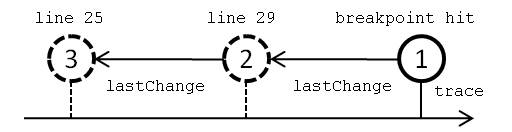
\includegraphics{5-example-points.jpg}
\caption{The examined points before locating the defect.}
\label{fig:example-points}
\end{figure}

\begin{figure*}[htp]

\subfigure[A screen shot of the Firebug debugger while running the example code from Fig.~\ref{fig:example2}. The Script
  panel is selected; it gives access to
  all loaded source files and allows breakpoints to be set on lines. In this
  figure, the execution is paused at line 22 by a regular
  breakpoint. The Watch panel at the right shows the program state at
  the paused
  point. ]{\label{fig:example1}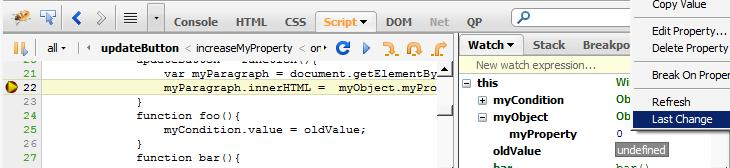
\includegraphics[width=1.0\textwidth,
    height=.19\textheight]{1-bp22.jpg}}

\subfigure[Developer can query \textit{lastChange} on a value by right-clicking 
on the
  value of \texttt{myProperty}.]{\label{fig:example2}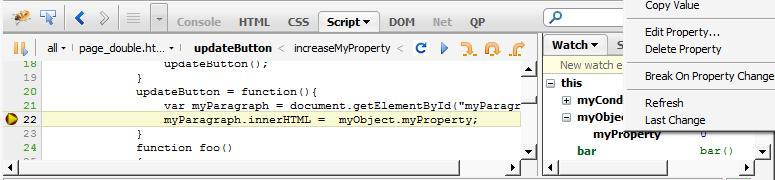
\includegraphics[width=1.0\textwidth,
    height=.19\textheight]{2-bp22-lastChange.jpg}}

\subfigure[The result of \textit{lastChange} query for
  \texttt{myObject.myProperty}. The left panel, QP, shows the source
  code at the point of \textit{lastChange}; The right panel,
  TraceData, shows the collected data at the
  point.]{\label{fig:example3}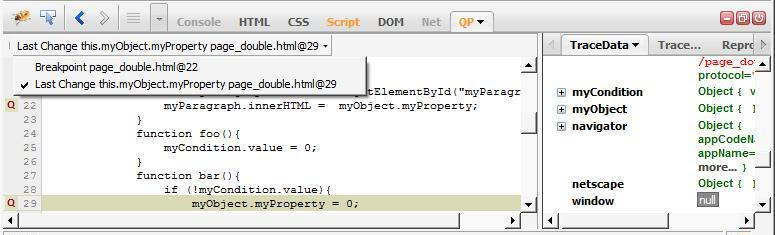
\includegraphics[width=1.0\textwidth,
    height=.23\textheight]{3-lastChange.jpg}}

\subfigure[The result of \textit{lastChange} query for
  \texttt{myCondition.value}. The opened list on the top of the left
  panel shows the visited execution points. Clicking on each point in
  the list shows the corresponding code and
  data.]{\label{fig:example4}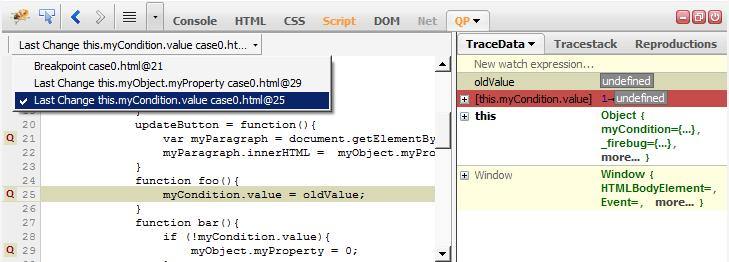
\includegraphics[width=1.0\textwidth,
    height=.23\textheight]{4-lastChange2.jpg}}

\caption{The stages of locating the defect using \textit{lastChange} feature.}
\label{fig:lastChange}
\end{figure*}


Notice that in our example, \textit{lastChange} combines some aspects
of breakpoint and of log-based debugging. Like breakpoint debugging,
the developer re-executes a live runtime without changing the source
and without a special execution environment beyond the debugger. The
state of the program memory and the call stack are available at the
lastChange point. Like log-based debugging, the program state and the
call stack are recorded during program execution. We can't halt the
program at \textit{lastChange} because we don't know which is the last
one until we return to the original breakpoint. (In section 5 we
discuss cases were it is possible to pause at lines of \textit{lastChange}).

%---------------------------------------------------------------------------------------------------
\section{\textit{lastChange} Algorithm}

The \textit{lastChange} algorithm is based on program re-execution of
a program halted on a breakpoint. The breakpoint hit becomes the
\textit{reproduction point}. The algorithm starts when developer
examines the program state at a breakpoint hit and asks for the
\textit{lastChange} of a value.  Debugger sets hooks (a callback
function dependent upon the underlying runtime) on all instructions
that might be the result of \textit{lastChange} query. Then the
debugger re-executes the program and every time the hook hits it
checks for a \textit{change event}. In the case of a change, it stores
part of the program state values.  Once the execution reaches the
reproduction point, it analyzes the collected data and shows the
result.  The program state at the execution point for the last change
event is the \textit{lastChange}.

While \textit{lastChange} itself is not a different kind 'breakpoint',
all of the assumptions developers already have for breakpoints hold
for \textit{lastChange}. In particular the re-execution is just the
same operation developers use to debug with breakpoints. Because
\textit{lastChange} dramatically reduces the developers work in
setting and removing breakpoints, the re-execution step will become a
much larege fraction of the debug time. Therefore automatic mechanisms
for re-execution will be corresponding more valuable for debugging
with \textit{lastChange}.

As we described in the preceding section, a \textit{lastChange} query can
be performed on the result of another \textit{lastChange} query. If we
name the reproduction point \textit{R}, we can write the first
\textit{lastChange} in the introductory example in this form:
\textit{lastChange(R, myObject.myProperty)}. It means that this query
is defined at \textit{R}. If we name the result of this query
\textit{A}, we can write the second \textit{lastChange} in this form:
\textit{lastChange(A, myCondition.value)}. In this way, a sequence of
\textit{lastChange} queries with any length can be defined.

\textit{lastChange} can be called on two different types of values: An
object property or a variable value. Three different variations of the
algorithm are required, one for object property and two more depending
upon the scope of a variable.

\subsection{\textit{lastChange} on object propery}
To simplify the algorithm explanation and defer technical details, we
define two basic operations and later we explain the details of these
two operations. The first opertion is \texttt{objectId()}: given a
JavaScript object it returns an integer as its identifier. This
identifier is unique to the object during one execution. The second
operation is \texttt{setPropertyChangeHook()}: given a function and a
string, the function is called whenever a property changes and its
name matches the string For example, if the property might be
\texttt{foo} so changes to \texttt{bar.foo} or \texttt{baz.foo} would
call the function.  The callback function receives a reference to the
owner of \texttt{foo}.


\begin{figure}[htp]
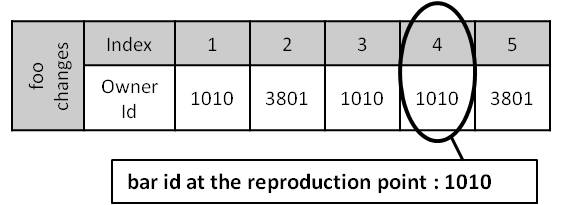
\includegraphics[width=.48\textwidth]{6-foo-changes1.jpg}
\caption{The list of property \texttt{foo} change events and
  \texttt{bar} id at the reproduction point which identifies the last
  change of \texttt{bar.foo} in the list. Column 3 is also a change of
  the object we want to study, id 1010, but it is not the last change;
  Column 5 is also a change of a property \texttt{foo} but its not for
  the object we are interested in.}
\label{fig:foo-changes1}
\end{figure}

To see how these functions work, suppose the developer asks for the
last change of \texttt{bar.foo} at the reproduction point in a
program. The debugger calls \texttt{setPropertyChangeHook()} with
\texttt{foo} as the property name and re-executes the
program. Whenever \texttt{foo} changes and the callback function is to
be called, debugger first calls \texttt{objectId()} on the
\texttt{foo} owner object. Then it stores this owner id, the stack
frame locations, and other state values in scope at the call point.
Whenever the execution reaches the reproduction point the debugger
looks at the history of \texttt{foo} changes and finds the last
\texttt{foo} change with the same object id as \texttt{bar} id at the
reproduction point. Figure ~\ref{fig:foo-changes1} shows the list of
property \texttt{foo} change events in a hypothetical
execution. \texttt{bar} id at the reproduction point is 1010, so the
last change of \texttt{bar.foo} is the fourth column.  By using an
object id instead of an object reference we allow the garbage
collector to reclaim the space for dead objects just at would in the
absence of the debugger.

\subsection{\textit{lastChange} on variable} 
In JavaScript, every frame has a scope chain and every available
variable in the frame comes from one of the scopes in the frame's
scope chain. Once developer asks for the last change of variable
\texttt{foo} at the reproduction point, debugger first determines the
variable's scope as follows: it iterates over the scopes in the scope
chain and the first scope which has a variable with the same name is
the variable's scope. There are five different scope types: local,
global, \texttt{with}, closure and \texttt{catch}. We explain these
cases in two groups.


\subsubsection{global and \texttt{with} scopes}
Global scope is the the most outer scope in the scope chain and it is
also refered to as the global object (the \texttt{window}
object in Web pages). This scope is a regular JavaScript object and therefore every
global variable is a property of global object. Similarly,
 \texttt{with} scopes are also regular objects. A \texttt{with}
scope is created by a \texttt{with()} block with an object as the
parameter. Every property of this parameter object is available inside the
block as a variable. Debugger treats the case where variable's scope
is global or \texttt{with}, like \textit{lastChange} on an object
property.

\subsubsection{local, closure and \texttt{catch} scopes}
Local scope refers to the most nested scope in the scope
chain. Closure scope refers to the scope which is created once a
function is defined. Catch scope is the scope created in the catch
block of try-catch statements and contains the exception
variable. These scopes are not necessarily regular JavaScript
objects. Therefore, to track changes to a variable in these scopes we
need a different approach.

All scopes in the scope chains come from blocks around the executing code.
Comparing the scope chain and the script we can identify the code block     % perhaps needs more explanation
(script) corresponding to the variable scope. Similar to \textit{lastChange} 
on object property, we define two basic operations \texttt{scopeId()} and
\texttt{setVariableChangeHook()}. The first one given an scope and its defining 
block(script) returns an integer as the scope's identifier. The second one 
given a callback function, a block(script) and a variable name, the function is called
whenever the variable is changed. After developer asks for the \textit{lastChange}
on a variable, in re-exeuction whenever the script is loaded, \texttt{setVariableChangeHook()}
is called. Every time the callback function is called a new change 
event is inserted to the list of change events.


\begin{figure}[htp]
\begin{verbatim}

  function f(){
    var x;
    x++;
    if (!stop) f();
  }

Sample Trace:

   f()
A  |  x changes; 
   |  f()
   |  |  x changes;
   |  |  f()
B  |  |  |  x changes; 
C  |  ?

\end{verbatim}
\caption{A recursive call trace demonstrates the need for scope
  id. Querying \textit{lastChange} on \texttt{x} at point C should
  return point A not B.}
\label{fig:recursive}
\end{figure}

Figure ~\ref{fig:recursive} demonstrates a case that the same variable
\texttt{x} is changed several times but in different scopes due to the
recursive calls. Without considering the scopes calling \textit{lastChange(x)}
at point C will return point B while the right answer is point A. Using
\texttt{scopId()} operation, the scope id is also stored at every variable
change event.
 
After developer asks for the \textit{lastChange} on a variable, 
Once the execution reaches the reproduction point, using variable's scope
id, the last change is recognized (Figure ~\ref{fig:foo-changes2}).

\begin{figure}[htp]
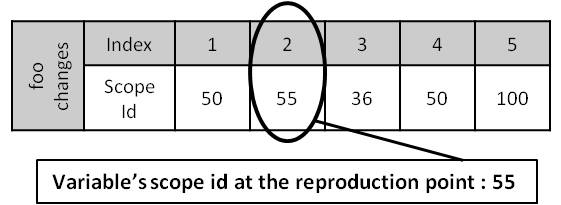
\includegraphics[width=.48\textwidth]{7-foo-changes2.jpg}
\caption{The list of variable \texttt{foo} change events and the
  \texttt{foo}'s scope id at the reproduction point which identifies
  the last change.}
\label{fig:foo-changes2}
\end{figure}

 
\subsection{\textit{lastChange} on \textit{lastChange}}
The algorithm we explained so far needs an enhancement to support
longer sequence of \textit{lastChange}s. We explain first the issue
and then the solution. Consider the following points:

\begin{center}
\textit{
 point A : the reproduction point \\
 point B : lastChange(A, bar.x) \\
 point C : lastChange(B, baz.y) 
 }
 \end{center}
According to the algorithm explained in the previous section none of
the points B and C can be identified before reaching point
A. Therefore, all \texttt{x} changes for point B and all \texttt{y}
changes for point C are stored. Once the execution reaches point A,
and the exact \texttt{bar} id reveals, point B can be identified among
the change events in the history of \texttt{x} changes. The problem
arises in recognizing point C. To recognize point C, we need
\texttt{baz} id at point B, but B is a past program state, and
\texttt{baz} id has not been collected at this point.

To address this issue, we use Algorithm \ref{dependency-analysis}, to
create the list of additional data should be collected at a change
event. This algorithm does does a dependency analysis between all
\textit{lastChange} queries and computes the list additional data
required to be collected at each change event. For example in the
mentioned case, \texttt{baz} id-if it is available- should be
collected at all points \texttt{x} changes. Having this additional
data, locating point C, using \texttt{baz} id at point B is
straightforward (Figure ~\ref{fig:lastchange-lastchange}).

\begin{algorithm}
\caption{\textit{lastChange} queries dependency analysis.}
\label{dependency-analysis}
\begin{algorithmic}

\FOR{$q$ in $queries$} 
 \FOR {$p$ is defined at the $q$ result}
   \IF {$p$ is a lastChange on object property} 
     \STATE the property owner id should be stored at $q$ change events. 
   \ELSIF {$p$ is a lastChange on variable} 
     \STATE the variable scope id should be stored at $q$ change events.
	 \ENDIF 
 \ENDFOR 
\ENDFOR

\end{algorithmic}
\end{algorithm}

\begin{figure}[htp]
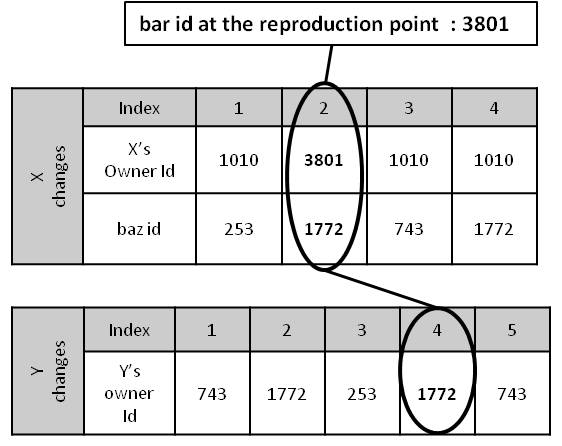
\includegraphics[width=.48\textwidth]{8-lastchange-lastchange.jpg}
\caption{The list of change events stored for locating point B, the
  \textit{lastChange} of \texttt{bar.x} at the reproduction point, and
  point C, the \textit{lastChange} of \texttt{baz.y} at point B.}
\label{fig:lastchange-lastchange}
\end{figure}




%---------------------------------------------------------------------------------------------------
\section{JavaScript implementation}
To verify the \textit{lastChange} algorithm we
implemented it in an extension to the Firebug
JavaScript debugger\cite{firebug-version-1.6}. 
Firebug itself is an extension of the Firefox browser\cite{firefox-version-3.6}. The Firefox
JavaScript engine provides a JavaScript debugging interface and
\textit{Querypointer} is developed over this interface. 

\subsection{\texttt{objectId()} operation}
\texttt{objectId(obj)} first checks the argument \texttt{obj} for a property \texttt{\_objectId}.
It returns the value if this property is already defined,
otherwise it generates a new id and sets this property. The value of the id is simply an integer incremented 
for each new \texttt{\_objectId} needed. To set %\textit{CHECK THAT} 
the property, we call the \texttt{defineProperty} standard JavaScript
function. \texttt{defineProperty} receives an argument which specifies
whether the property is enumerable or not. By setting the enumerable
field \texttt{false} for \texttt{\_objectId}, this property will not
apear in \texttt{for(property in object)} loops and therfore has no
effect on the program execution. Note that \texttt{\_objectId} is
not set for all objects but only those objects that need an id.

\subsection{\texttt{setPropertyChangeHook()} operation}
The Firefox JavaScript engine supports watching property changes in an
object. Every object has a function \texttt{watch(propName, callback)}
which receives two parameters, a property name and function.  Whenever
the property with the given name changes, the \texttt{callback} function is
called. The hook set by this function remains enabled even if the
property is deleted and defined again. 

For our purposes, the \texttt{watch()} function only covers the case
of global object properties. At the beginning of execution, no object
excepting the global object is available. Therefore we defined and
implemented \texttt{setPropertyChangeHook()} to work in the rest of
the cases. 

The Firefox JavaScript engine does not current support
\texttt{setPropertyChangeHook()} (see however \cite{bugzilla}).  For
the our \textit{lastChange} prototype we created a version of
\texttt{setPropertyChangeHook()} using only features of the current
engine.  The basic strategy is to get a reference to the object just
after its creation, then use \texttt{watch()} function to monitor
property changes in the object.  Setting a flag into the Firefox
JavaScript engine we can get file URL and line number for each object
creation (e.g., myFile.js, line 24). We set a breakpoint on this line
and analyze the source code to determine which object was created.
 
\subsection{Tracking object creation}
The only data we have is the object creation location including the
file url and the line number and the goal is to get a reference to
this object. Although in the most regular cases we have only one
statement and one object creation in a line, there are cases that more
than one object might be created in a line. There is no way to
recognize the interesting object among these new objects. So instead
of one object, we monitor all new objects created in the line.

An object might be created by one of these statements: An object
initializer(\texttt{\{...\}}) or \textit{new} operator (\texttt{new
  constructor()}) or function objects which can be created by
\texttt{function()} statement. By parsing the source code we can
easily recognize the statements create an object. The next step is
getting a reference to the new object.

The new object can be assigned to an object property or variable by
\texttt{=}. In these cases we keep the assignee statement at the left
side. The idea is that we create a list of assignee statements that
the new objects are assigned to them. We set a hook on the creation
line. Once the hook hits, we evaluate all statements. Then we do
stepping(step-over) and after each step we evaluate the
statements. Every statement which has a new value, we consider the new
value-if it is an object-as a new object. For example in Figure
~\ref{fig:objectCreation}(a), if the creation line number is 20, we
have only one statement which creates a new object and it is assigned
to \texttt{x.y}.

The new object can also be set as the property of a parent object by
\texttt{:}. This case is also treated similar to previous case. The
only difference is that the full path of property from the root parent
in the local scope should be considered as the assignee statement. For
example in Figure ~\ref{fig:objectCreation}(b), if the creation line
is 20, we keep \texttt{parentObject.newObject}. In this case stepping
should be continued until the end of line 22 for getting a reference
to the created new object.

There is another case for new objects and when they are passed as
arguments to other functions ~\ref{fig:objectCreation}(c). In these
cases instead of step-over we use step-in and we get the corresponding
argument as a new object.

%The algorithm is not complete and it is tried to support more and more cases

\begin{figure}[htp]
\begin{verbatim}
(a) Case 1:
20 x.y = new myConstructor();

(b) Case 2:
19  parentObject = {
20   	  newObject : {
21  			x : 5
22  }}

(c) Case 3:
20 myFunction({myProperty:5});
 
\end{verbatim}
\caption{Examples of three types of JavaScript object creatin statements.}
\label{fig:objectCreation}
\end{figure}


\subsection{\texttt{scopeId()} operation}
The scope id is kept as a variable with name \texttt{\_scopeId} in the
scope. We explained that we set a hook at the first instruction of the
function which defines the variable. Once this hook hits,
\texttt{\_scopeId} is set by calling JavaScript's dynamic compilation function \texttt{eval()}. For
example, executing \texttt{eval( var \_scopeId = 10)} creates a
variable with name \texttt{\_scopeId} and value \texttt{10} in the
scope of the \texttt{eval()} call, which is our interesting scope.

\subsection{\texttt{setVariableChangeHook()} operation}
Only operations in the scope of these varibles can change their value; 
that includes the defining scope and scopes nested inside of them.
For example in Figure ~\ref{fig:js-closure}, variable \texttt{var1} in line 11 can only be
changed in lines 10 to 23. Therefore, after locating the function in
which the variable is defined, it is enough to parse the code inside
the function block and set a hook on all lines where the variable is
assigned a new value. 
We also set a hook at the first line of the function which is
corresponding to the line variable is defined. In Figure
~\ref{fig:js-closure}, if the execution is paused at line 17 and the
last change of \texttt{var1} is queried, two hooks on lines 16 and 17
will be set, but if the execution is paused at line 20 , four hooks on
lines 11, 12, 14, 20 will be set. These two cases are different due
the fact that \texttt{var1} in \texttt{firstChild} is a local variable
but in \texttt{secondChild} is a closure variable.

\begin{figure}[htp]
\begin{verbatim}
10  function parent(){
11    var var1;
12    var1 = ...;
13    function myfun(){
14      var1 = ...;
15      function firstChild(){
16       	var var1;
17        var1 = ...;
18      }  
19      function secondChild(){
20        var1 = ...;			      
21      }
22    }  
23  }    
\end{verbatim}
\caption{Sample JavaScript code demonstrating local and clousure variables.}
\label{fig:js-closure}
\end{figure}
  

\section{Discussion}

We have presented the \texttt{lastChange} algorithm and describe our
prototype implementation. Now we want to convince you that the
algorithm has practical value. Ultimately, practical value can only be
proven by developers in the field using the technique. This paper is
one step to convince implementers to put \texttt{lastChange} in the
field.  Thus our goal here is a persausive argument.

The key ingredients in our argument are: 
\begin{enumerate}
   \item developers need an operation like \texttt{lastChange}, 
   \item developers can learn to use \texttt{lastChange}, 
   \item practical implementations are feasible with modest
invested development time,
   \item in most cases \texttt{lastChange} will be much faster than current alternatives,
   \item the worst cases are not more common or more painful than
alternatives.
\end{enumerate}

\subsection{developers need an operation like \protect\texttt{lastChange} }

We have shown how \texttt{lastChange} identifies the prior point in
program execution where a program state value changes. Is it something
the developer needs to do?  Since ultimately programs are just
transformation of state values, debugging is ultimately backtracking
to find defects in program state change.  When a developer halts a
program on a breakpoint they have three kinds of information: a model
of the program in their head, a call stack showing what part of the
program is halted, and the state at that point (a combination of the
debugger's view of the program internal state and the output of the
program up to this point of execution). If the model does not match
the call stack or if no value in the viewable program state aligns
with the developers model for this point in execution, the developer
will seek another view by changing the breakpoint or the input
data. If a value appears incorrect, they may have a flash of insight
and know the defect. Otherwise they need to figure out what operation
causes the incorrect value. Thus \texttt{lastChange} addresses a key
part of the debugging process.

\subsection{developers can learn to use \protect\texttt{lastChange}}

If \texttt{lastChange} could be useful, can developers figure out how
to use it? We hope that our prototype demonstrates that
\texttt{lastChange} can be easily activated by operations on the
graphical representation of erroneous data in a debugger. Intepreting
the results should be only slightly more difficult. We designed the
user interface for the results from \texttt{lastChange} to resemble
the results from a breakpoint, with the source code of the change
point highlighted and the state of the program presented the way state
is presented from a breakpoint. Based on this user interface, we
believe developers can start to use \texttt{lastChange} with minimal
training. Of course developers may initially confuse the result of
\texttt{lastChange} with being halted in a debugger at the point of
last change. The value of the result will motivate them to clarify the
issue.

\subsection{practical implementations are feasible}

We described our prototype implementation in Sec. 4. A fully usable
implementation would require access to the object id at the point of
object creation and \texttt{setPropertyChangeHook()}. Many
object-oriented runtimes provide object identifiers\cite{} and some
provide access to object creation\cite{}. In the particular case of
the Firefox Web browser we used for our prototype, the primary barrier
to practical implementation would likely be integration with the
increasingly sophisticated just in time compilers\cite{}. 

\subsection{in most cases \protect\texttt{lastChange} will be much faster than current alternatives}

When developers try \texttt{lastChange}, will they get results fast
enough to benefit? While we only used our prototype on toy programs,
\textit{lastChange} seemed as fast as re-execution.  Recall that we
insert additional code through debugger callbacks, then re-execute the
program. The additional code we insert is proportional (in our
JavaScript algorithm) to 1) the number of places a property or
variable with a given name is changed, 2) the number of places objects
are created. (Something about the likely overhead in Firefox).

For comparison we should use the practical alternative: developers
setting breakpoints. For the vast majority of programs, a developer
will take much more time to set one breakpoint than
\texttt{lastChange} would add. But typically the developer may not
guess the point of last change. They must then ponder another
breakpoint, and re-execution. 

We could also compare to solutions based on logging or tracing. Manual
logging has very high overhead: the developer must add code, debug
that added code, then analyze the log. (To be fair, the log can become
a permenant debugging aid.) Automatic logging as we discussion in
\secref{related} causes about one or two orders of magnitude slow down. 

\subsection{the worst cases are not more common or more painful than alternatives}

Finally we consider the worst cases: what about code that changes
objects in long running loops? Every time through the loop we incur
the call back overhead; if the loop itself has relatively little code
the overhead could be very large; if the loop computation is a
significant fraction of the full program, the slowdown would be
enormous. 

Of course breakpoints are not feasible in these cases and logging
becomes unyieldy. Since automatic logging solutions are highly tuned,
their overhead in this case will likely be much less than
\texttt{lastChange}. On the other hand, \texttt{lastChange} integrates
with an interactive debugger and detecting that we are in a high
overhead loop is simply a matter of checking our internal counter. In
such unusual cases we may simply offer the developer the option of
studying the loop code then omitting it from \texttt{lastChange}
operations. As a practical result, this is no different from similar
issues developers face with any debugger today: occasionally a
debugger causes too much overhead to be useful for debugging. On
balance we think \texttt{lastChange} will rarely encounter these kinds
of issues.

%---------------------------------------------------------------------------------------------------
\subsection{Reproducible Non-deterministic Execution}

By construction \textit{lastChange} works whenever conventional
breakpoint debugging works. By that we mean that, since we use
conventional breakpoint debugging technology under the covers,
\textit{lastChange} works whenever breakpoint debugging
works. However, there are cases where breakpoint debugging fails but
\textit{lastChange} works.  These are cases of \textit{reproducible
  non-deterministic} execution.

A bug is \textit{reproducible} for a developer when the developer can
start from a determined initial state, operate on the program with a
list of actions, and reproduce the symptoms of the bug. The details of
the execution can change each time we re-execute the buggy program,
but the buggy result is the same.  The reproducibility of the bug
means that the defect is very unlikely to depend on the order of
events during the execution. When the developer selects a value and
asks for \textit{lastChange}, they are expressing an hyptothesis that
the value is related to the defect. Therefore the reproducibility of
the bug makes it very unlikely that the \textit{lastChange} will
depend upon order of events during execution.

Since \textit{lastChange} does not rely on determinism, some bugs that
confound breakpoint debuggers will be easier to find with
\textit{lastChange}.  Consider the following example.
Figure ~\ref{fig:counter-example} shows a function with processes an
array. The array contains numbers except one itme which is
\texttt{undefined} and it causes a bug in line 30. There is a call to
\texttt{randomPermutation} function in line 11 which randomly
permutates the array item. So at every execution the
\texttt{undefined} item will be in a new place. Calling
\textit{lastChange} on \texttt{x} at the place bug happens, gives a
point which shows line 14. Although this point exists at every
re-execution but it can not be identified by a conditional breakpoint.

\begin{figure}[htp]
\begin{verbatim}
10 function randomProcess(array){
11   randomPermutation(array);
12   var x, y;
13   for (var i=0 ; i<array.length ; i++){
14      x = array[i]
...
30      y = x+1;
31   }
32 }
\end{verbatim}
\caption{A counter-example for transforming \textit{lastChange} to a conditional breakpoint.}
\label{fig:counter-example}
\end{figure}
 

Thus in the case of a non-deterministic program, a \textit{lastChange}
is not equivalent to any series of conventional watchpoints or
breakpoints. The extra power of \textit{lastChange} derives from its
analysis of the entire execution up to the reproduction point and its
memory of previous work on the defect.  Each time we re-execute a
non-deterministic program, the details of execution instruction order
may change. For example, if we record the source code lines every time
a conventional watchpoint hits, the record may differ each time we
re-execute. But \textit{lastChange} does not ask the developer to
consider these single points.  Rather we analyze all of the
watchpoints in an entire execution at the reproduction point where we
know the defect has already occured and only show the final result to
the developer.

Of course there can be cases where the defect is reproducible but the
value from \textit{lastChange} is not. As in conventional breakpoint
debugging, we can only determine this empirically, by observing
multiple executions with different values. Unlike conventionaly
breakpoint debugging, implementations of \textit{lastChange} readily
aid in detecting such cases: as we work back through a series of
\textit{lastChange} requests we can compare values with previous
executions. Different values on different executions will signal that
the execution is not deterministic. In future we hope to compare
queries from successive executions as a tool for learning about
non-deterministic executions.

\subsection{Execution reproduction}
Although execution reproduction is basicly should be provided by the
developer, we tried to devise some automatic way which reproduces the
execution. In \textit{Querypointer}, develooper can directly provide a
test case which reproduces the execution. It is also possible to use
two automatic reproduction option: record-replay or local-reproduction
.

Two elements should be carefully considered in execution
reproduction. First, the initial state should be the same as previous
execution. Second, the similar actions and events should be applied to
the program during the execution. In Record-replay approach, debugger
stores the initial page url and user actions and during replay phase,
opens the same url and simulates user actions. In the local
reproduction approach, debugger calls the funtion on the bottom of
stack with the same parameters. The idea behind local-reproduction is
that in many web pages it is enough to replay the event to reproduce
the bug. While record-replay approach gives better warranty about the
same initial states, the local-reproudction gives us shorter
cycles. It is also possible to uses thes approaches in
combination. For example, debugger locally reproduce the execution and
if it couldn't find the answer, reproduce the whole execution by
record-replay.
% should we talk about counting breakpoint hits for stopping at the right place?

\subsection{Data collection and presentation}
So far, we talked about the data collected at change events for
\textit{lastChange} algorithm. However, if developer needs to explore
the program state at a given point, more data is required. It is
possible to postpone data collection until user requests. It is also
possible to collect the list of available
variable. \textit{Querypointer} collects data in one level depth. More
data will be collected upon the developer's request by re-execution.

We needed to build an interface to different execution points which
are presented at the same time. The current \textit{Querypointer}
interface resembles the script panel interface while it keeps the
history of navigation.

\subsection{Reproduction point}

\section{Evaluation}
\subsection{\textit{lastChange} effectiveness}

\subsection{Execution overhead analysis}
If we assume that the total number of instructions in an execution is
$n$ and $m$ change event happens during one execution and for every
change event $k$ additionial instructions should be executed, the
execution overhead of our approach is $mk/n$. For $m=10^3$, $k=10^2$
and $n=10^{10}$ the overhead is very low and about $10^{-5}$.

\section{Related Work}

\textit{lastChange} functionality supports obtaining information about
the execution state logically earlier in the control flow. This
support resembles a mixture of replay-based and logging-based
debugging. Replay-based approaches capture limited data during
execution and replay the bug-gy execution to reach past points. In
contrast, logging-based approaches collect enough data during
execution to relieve developer from re-execution. Replay-based
approaches impose much less runtime overhead (about two orders of
magnitudes) comparing to logging-based appproches. However, developer
has to re-execute the buggy execution several
times. \textit{lastChange} functionality collects data on re-execution
but this data is limited to the current queries of developer.

Among replay-based debuggers we compare to bdb \cite{Boothe} and
reverse watchpoint \cite{Maruyama}.  A bidirectional C debugger, bdb
employs a step counter to locate the requested point from the
beginning of execution. It relies on deterministic execution replay
(i.e., the same sequence of instructions in re-execution) and records
the results of non-deterministic system calls and re-injects them into
the program when it is replayed. It makes use of checkpoints to reduce
the time needed for re-execution.  Reverse watchpoint, is proposed by
Maruyama et al., analyses the execution and moves the debugger to the
last write access of a selected variable by re-executing the program
from the \cite{Maruyama}.  Similar to bdb it relies on deterministic
replay and uses a counter to correctly locate a point in the next
execution. The main disadvantage of these appraoches is requiring the
exactly the same executions. Even one instruction difference between
in two executions leads to wrong results. This requirement is that
much restricting that after ten years from bdb paper publication,
there is no newer implementation of this idea. On the other hand,
\textit{lastChange} doesn't require any special feature in the
re-rexecution and it is fit to everyday's developers' debugging
practice.

Among logging-based approaches are "omniscient" debuggers
ODB\cite{Lewis} and Unstuck[]. Omniscient debuggers have been proposed
as a solution for the problems of breakpoint-debugging. Both
approaches keep the log history in memory and hence can only record
and store the complete history for a short period of time. These
debuggers record all the events that occur during the buggy execution
and later let the developer to navigate through the obtained execution
log. In this approach there is no execution to resume: moving
backwards in the log can be similar to moving forwards. Omniscient
debuggers suffer from a different set of issues. First, the recording
step is time expensive and it should be repeated in case of changes in
program. Second, the execution log cannot fully replace the live
execution. There are other aspects of execution (e.g., program user
interface, file system, database tables, etc.) which are also
important in debugging and are not available to the developer in
omniscient debuggers. Third, querying collected data (e.g., to restore
the program state at a certain point) may not be efficient enough for
debugging of realistic programs.

A more scalable approach has been proposed by Pothier et
al. \cite{Pothier}. Their back-in-time debugger, TOD, addresses the
space problem by storing execution events in a distributed
database. Comparing to Omniscient debuggers our approach is
lightweight and more flexible. Developer can start debugging just
after reproducing bug without a capturing step.  Changing inputs or
environment settings and re-executing to investigate the bug works as
in conventional breakpoint debuggers.

Two new directions in logging debuggers explore more detailed use of
the log and more effective logging approaches. WhyLine\cite{Ko}
provides visual interface to collected runtime information and let
developer to move on execution log using queries expressed in terms of
the programming objects. WhyLine stores the program user in-terface in
addition to program trace and provides answers to why and why not
questions to the user. Jive\cite{Czyz} depicts the history of
execution by a sequence diagram and lets user to query on events
database. Both tools suffer from similar issues with omniscient
debuggers;
%both provide models for extending Querypoint debugging to obtain a better user interface while retaining the flexible conven-tional replay model of debugging.  

A recent work by Lienhard et al.\cite{Lienhard} suggests virtual
machine level support for keeping the object flow. It rep-laces every
object reference with an alias object which keeps the history of
changes to the object reference. In this way, when an object is
collected by garbage collector, its track of changes (if it is not
referenced by other alias-es) will be also collected. Though this
approach incurs less runtime overhead (7 times to 115 times) in
comparison to omniscient debuggers, it adds memory
overhead. Querypoint debugging uses re-executions to gather
infor-mation requested by the developer: the memory overhead depends
on the query not the entire program. Moreover, the Lienhard et
al. debugger significantly changes the virtual machine, while our
approach is a generalization to conditional breakpoints and available
debugger infrastructure can be adapted to support it.
 
\textit{lastChange} functionality does rely on a conventional
breakpoint to begin queries, a requirement not shared by full logging
solutions.  Here we leverage past experience of developers, but there
are also new tools [] to help with this problem in the case of
graphical and event based systems.


\section{Conclusions and Future Work}



% We recommend abbrvnat bibliography style.

\bibliographystyle{abbrvnat}

% The bibliography should be embedded for final submission.

\begin{thebibliography}{10}
\softraggedright

\bibitem[Bond(2007)]{Bond}
M.D. Bond, N. Nethercote, S.W. Kent, S.Z. Guyer, and K.S. McKinley. \newblock Tracking bad apples: reporting the origin of null and undefined value errors.
\newblock In \emph{22nd annual ACM SIGPLAN conference on Object-oriented programming, systems, languages, and applications(OOPSLA)},
October, 2007.

\bibitem[Boothe(2000)]{Boothe}
B. Boothe. \newblock Efficient algorithms for bidirectional debugging.
\newblock In \emph{Conference on Programming Language Design and Implementation(PLDI)},
June, 2000.

\bibitem[Czyz(2007)]{Czyz}
J.K. Czyz, and B. Jayaraman. \newblock Declarative and visual debugging in Eclipse.
\newblock In \emph{OOPSLA workshop on eclipse technology eXchange},
October, 2007.

\bibitem[Firebug(2010)]{Firebug}
Firebug. \newblock http://getfirebug.com.

\bibitem[Ko(2008)]{Ko}
A.J. Ko, and B.A. Myers. \newblock Debugging reinvented: asking and answering why and why not questions about program behavior.
\newblock In \emph{30th international conference on Software engineering(ICSE)},
May, 2008.

\bibitem[LaToza(2006)]{LaToza}
T.D. LaToza, G. Venolia, and R. DeLine. \newblock Maintaining mental models: a study of developer work habits
\newblock In \emph{28th international conference on Software engineering(ICSE)},
May, 2006.

\bibitem[Lewis(2003)]{Lewis}
B. Lewis, and M. Ducasse. \newblock Using events to debug Java programs backwards in time.
\newblock In \emph{Companion of the 18th annual ACM SIGPLAN conference on Object-oriented programming, systems, languages, and applications(OOPSLA)},
2003.

\bibitem[Lienhard(2008)]{Lienhard}
A. Lienhard, T. G\^{\i}rba, and O. Nierstrasz. \newblock Practical Object-Oriented Back-in-Time Debugging.
\newblock In \emph{22nd European conference on Object-Oriented Programming(ECOOP)},
July, 2008.

\bibitem[Maruyama(2003)]{Maruyama}
K. Maruyama, and T. Kazutaka. \newblock Debugging with Reverse Watchpoint.
\newblock In \emph{Proceedings of the Third International Conference on Quality Software},
2003.

\bibitem[Pothier(2007)]{Pothier}
G. Pothier, \'{E}. Tanter, and J. Piquer. \newblock Scalable omniscient debugging.
\newblock In \emph{22nd annual ACM SIGPLAN conference on Object-oriented programming, systems, languages, and applications(OOPSLA)},
October, 2007.


\end{thebibliography}

\end{document}
